\section{Aufbau und elektronische Beschaltung}
In Abbildung \eqref{fig:Aufbau} ist der schematische Aufbau des gesamten Gerätes aufgezeigt. Allerdings fehlen die Kühlung und die Blei-Burg für den Detektor und den Vorverstärker. Das Ziel des Aufbaus ist es einen Spannungsimpuls zu erzeugen der proportional zu der $\gamma$-Energie ist. Die benötigten Komponenten werden im folgenden beschrieben.

\begin{figure}
  \centering
  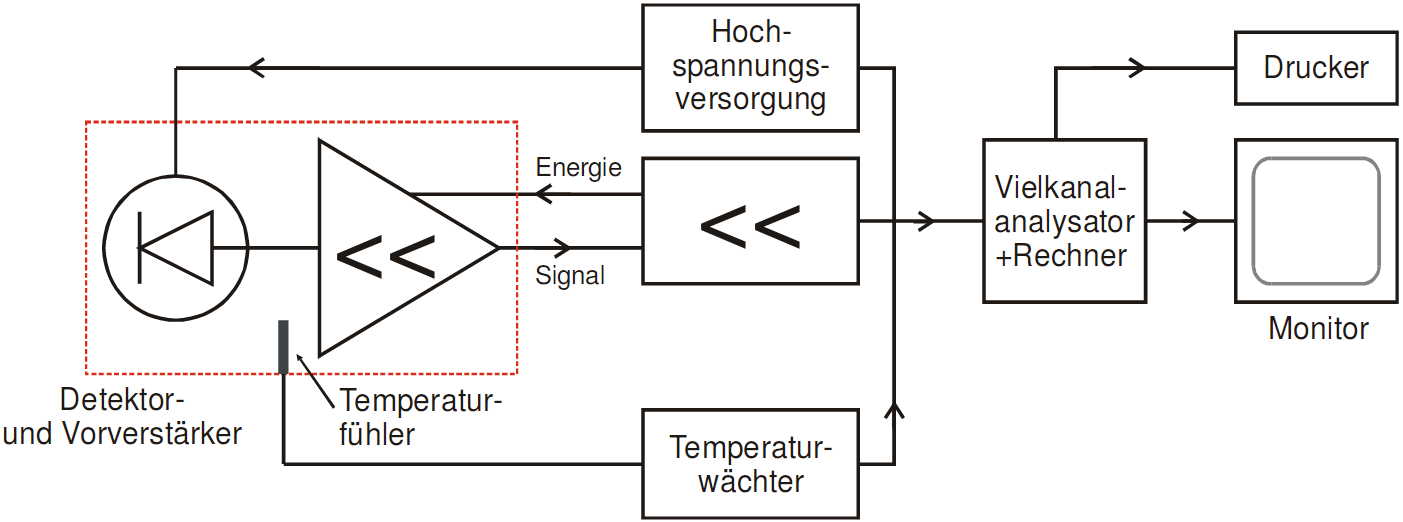
\includegraphics[width=\linewidth]{Bilder/Aufbau.png}
  \caption{Der schematische Aufbau des $\gamma$-Spektrometers ohne Kühlung \cite{V18}.}
  \label{fig:Aufbau}
\end{figure}

Der verwendete Detektor ist in Abbildung \eqref{fig:DetektorAufbau} skizziert. Der Germanium-Kristall hat die Gestalt eines Zylinders und ist von außen mit Lithium bedampft und von innen mit Gold. Dadurch ist der Kristall außen n-dotiert und innen p-dotiert. Der Pluspol für die Sperrspannung wird an der Lithium-Schicht angebracht. \\
Um den Kristall befindet sich eine Schutzhaube aus Aluminium. Diese schließt den Kristall Luftdicht ein, dadurch kann der Kristall nicht verunreinigt werden. Allerdings können wegen der Schutzhaube und der Lithium-Schicht nur $\gamma$-Energien größer als 40\,keV nachgewiesen werden.

\begin{figure}
  \centering
  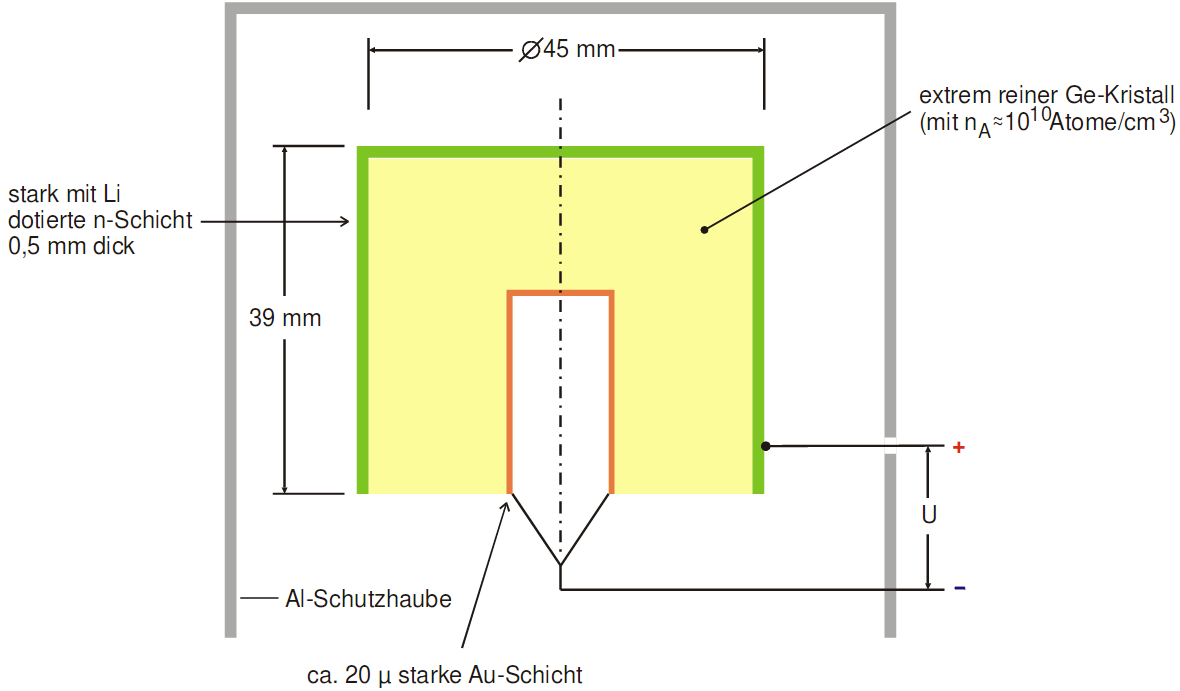
\includegraphics[width=\linewidth]{Bilder/Germanium-Detektor.png}
  \caption{Schematischer Aufbau eines koaxialen Reinst-Germanium-Detektors \cite{V18}.}
  \label{fig:DetektorAufbau}
\end{figure}

\begin{figure}
  \centering
  \includegraphics[width=\linewidth]{Bilder/Vorverstärker.png}
  \caption{Beschaltung eines Vorverstärkers im Reinst-Germanium-Detektor \cite{V18}.}
  \label{fig:Vorverstärker}
\end{figure}
















\section{Versuchsdurchführung}
